\documentclass[]{article}
\usepackage{lmodern}
\usepackage{amssymb,amsmath}
\usepackage{ifxetex,ifluatex}
\usepackage{fixltx2e} % provides \textsubscript
\ifnum 0\ifxetex 1\fi\ifluatex 1\fi=0 % if pdftex
  \usepackage[T1]{fontenc}
  \usepackage[utf8]{inputenc}
\else % if luatex or xelatex
  \ifxetex
    \usepackage{mathspec}
  \else
    \usepackage{fontspec}
  \fi
  \defaultfontfeatures{Ligatures=TeX,Scale=MatchLowercase}
\fi
% use upquote if available, for straight quotes in verbatim environments
\IfFileExists{upquote.sty}{\usepackage{upquote}}{}
% use microtype if available
\IfFileExists{microtype.sty}{%
\usepackage{microtype}
\UseMicrotypeSet[protrusion]{basicmath} % disable protrusion for tt fonts
}{}
\usepackage[margin=1in]{geometry}
\usepackage{hyperref}
\hypersetup{unicode=true,
            pdftitle={Tree size and hydraulic traits shape drought responses in a temperate broadleaf forest},
            pdfauthor={Ian McGregor, Ryan Helcoski, Norbert Kunert, Alan Tepley, Valentine Herrmann, Joseph Zailaa, Atticus Stovall, Neil Pederson, Lawren Sack, Krista Anderson-Teixeira},
            pdfborder={0 0 0},
            breaklinks=true}
\urlstyle{same}  % don't use monospace font for urls
\usepackage{natbib}
\bibliographystyle{apalike}
\usepackage{graphicx,grffile}
\makeatletter
\def\maxwidth{\ifdim\Gin@nat@width>\linewidth\linewidth\else\Gin@nat@width\fi}
\def\maxheight{\ifdim\Gin@nat@height>\textheight\textheight\else\Gin@nat@height\fi}
\makeatother
% Scale images if necessary, so that they will not overflow the page
% margins by default, and it is still possible to overwrite the defaults
% using explicit options in \includegraphics[width, height, ...]{}
\setkeys{Gin}{width=\maxwidth,height=\maxheight,keepaspectratio}
\IfFileExists{parskip.sty}{%
\usepackage{parskip}
}{% else
\setlength{\parindent}{0pt}
\setlength{\parskip}{6pt plus 2pt minus 1pt}
}
\setlength{\emergencystretch}{3em}  % prevent overfull lines
\providecommand{\tightlist}{%
  \setlength{\itemsep}{0pt}\setlength{\parskip}{0pt}}
\setcounter{secnumdepth}{0}
% Redefines (sub)paragraphs to behave more like sections
\ifx\paragraph\undefined\else
\let\oldparagraph\paragraph
\renewcommand{\paragraph}[1]{\oldparagraph{#1}\mbox{}}
\fi
\ifx\subparagraph\undefined\else
\let\oldsubparagraph\subparagraph
\renewcommand{\subparagraph}[1]{\oldsubparagraph{#1}\mbox{}}
\fi

%%% Use protect on footnotes to avoid problems with footnotes in titles
\let\rmarkdownfootnote\footnote%
\def\footnote{\protect\rmarkdownfootnote}

%%% Change title format to be more compact
\usepackage{titling}

% Create subtitle command for use in maketitle
\newcommand{\subtitle}[1]{
  \posttitle{
    \begin{center}\large#1\end{center}
    }
}

\setlength{\droptitle}{-2em}

  \title{Tree size and hydraulic traits shape drought responses in a temperate
broadleaf forest}
    \pretitle{\vspace{\droptitle}\centering\huge}
  \posttitle{\par}
    \author{Ian McGregor, Ryan Helcoski, Norbert Kunert, Alan Tepley, Valentine
Herrmann, Joseph Zailaa, Atticus Stovall, Neil Pederson, Lawren Sack,
Krista Anderson-Teixeira}
    \preauthor{\centering\large\emph}
  \postauthor{\par}
    \date{}
    \predate{}\postdate{}
  
\usepackage{booktabs}
\usepackage{longtable}
\usepackage{array}
\usepackage{multirow}
\usepackage{wrapfig}
\usepackage{float}
\usepackage{colortbl}
\usepackage{pdflscape}
\usepackage{tabu}
\usepackage{threeparttable}
\usepackage{threeparttablex}
\usepackage[normalem]{ulem}
\usepackage{makecell}
\usepackage{xcolor}

\usepackage{float}
\usepackage{booktabs}
\usepackage{pdflscape}
\newcommand{\blandscape}{\begin{landscape}}
\newcommand{\elandscape}{\end{landscape}}
\usepackage{caption}
\captionsetup[table]{font=small}
\captionsetup[figure]{font=small}
\captionsetup[table]{labelformat=empty}
\usepackage{dcolumn}

\begin{document}
\maketitle

\subsubsection{Summary}\label{summary}

Predicting forest responses to drought is an increasingly critical task
under climate change effects. Part of the problem is due to the lack of
studies analyzing the confluence of leaf hydraulic traits with
biophysical parameters. In this study, we analyze the interaction
between these two trait groups using forest census data from a 25.6-ha
ForestGEO plot in Virginia (USA). Drought periods were defined by both
Palmer Drought Severity Indices (PDSI) and their identification from
tree-ring records for 12 species representing 97\% of woody
productivity. Each drought scenario (1964-66, 1977, 1999), along with
the overall trend, was then tested against leaf hyraulic trait
measurements and microhabitat biophysical data. Individual-level growth
responses to the three individual droughts were stronger among taller
trees in dominant canopy positions, those in wetter microsites, and for
more drought-sensitive species as assessed by leaf traits (turgor loss
at less negative leaf water potential, greater shrinkage with leaf
dehydration), with substantial variation in the best predictor variables
across given droughts. We conclude that when droughts occur, large
dominant trees, drought-sensitive species, and individuals in wetter
microhabitats are likely to be most strongly affected.

\emph{The Summary for research papers, which must be usable as a stand-
alone document, must not exceed 200 words and should be organized using
four bullet points to indicate: (1) the research conducted, including
the rationale, (2) methods, (3) key results, and (4) the main
conclusion, including the key points of discussion. It should not
contain citations of other papers.}

\subsubsection{Introduction}\label{introduction}

Understanding how and why trees respond to drought is critical to
predicting forest drought responses and climate change feedbacks. (1
paragraph on this- I have lots of content on this and will add later.)

{[}Understanding forest responses to drought requires increased
functional understanding of the factors that confer individual-level
vulnerability or resistance.{]} Forests are diverse in terms of tree
sizes and functional traits, and it is known that trees varying in size
and functional traits respond differently to drought (e.g.,
\citep{bennett_larger_2015}; REFS). Therefore, in order to understand
whole-forest response to drought, we need a functional understanding of
how responses vary by tree size, microhabitat, and species. There are 3
fundamental questions that must be addressed:

\emph{First, what drives the observed tendency for large trees to suffer
more during drought?}\\
\citet{bennett_larger_2015} showed that in forests globally, large trees
suffer greater growth reductions during drought. However, this analysis
quantified tree size based on DBH, which has no direct mechanistic
meaning. This study proposed two major mechanisms (besides insects) for
the observed greater drougth growth reductions of large trees: (1)
inherently greater biophysical challenge of being tall; (2) greater
exposure of the crowns of large trees. Counteracting these effects, (3)
the larger root systems of larger trees may confer an advantage in terms
of allowing greater access to water, but it appears that this effect is
usually insufficient to offset the costs of height and/or crown
exposure.

Canopy trees have lower drought resistance because they are exposed to
higher solar radiation, greater wind speeds, and lower humidity.
Alternatively, the generally supressed status of subcanopy trees may be
insufficient to override the benefits of their buffered environment
during drought.

\emph{Second, how do species' traits - alone and in interaction with
tree size - influence drought response?} Analyzing drought responses on
the species level does not fully explain mechanisms and is not feasible
in diverse forests. The solution is a trait-based approach. Leaf
hydraulic traits hold more promise than more
commonly/traditionally-measured traits such as wood density and specific
leaf area (SLA)
(\href{https://besjournals.onlinelibrary.wiley.com/doi/abs/10.1111/1365-2435.13229}{Medeiros
et al. 2019}).

Commonly measured traits including wood density (REFS), leaf mass per
area \citep{abrams_adaptations_1990} \citep{guerfel_impacts_2009}, and
ring porosity (Elliot et al. 2015, Friedrichs et al. 2009) have been
linked to drought responses and likely correlated with drought
resistance in this forest. However, we hypothesize that leaf hydraulic
traits such as leaf area shrinkage upon dessication (PLA) and turgor
loss point (TLP), which are emerging as potentially more informative
traits but whose effect on drought resistance has never been tested
(CONFIRM), will prove better predictors.

Moreover, there may be an interaction between traits and tree size. It
is possible that the pattern observed by \citet{bennett_larger_2015}
could be caused by smaller trees being more drought resistant.
Alternatively, larger trees may have more drought-resistant traits as
adpatations to greater biophysical challenges.

\emph{Third, are responses similar or variable across individual drought
years?} Droughts are rarely explicitly defined in ecological studies
\citep{slette_how_2019}, yet no two droughts are the same.

We need to understand the the factors confirming drought vulnerability
or resistance not only for extreme droughts with dramatic impacts on
tree growth and mortality, which tend to dominate the literature
\citep{bennett_larger_2015} (REFS), but also for more modest but
frequent droughts--e.g., those with historical return intervals on the
order of a decade.

Here, we combine tree-ring records covering three droughts (1964-66,
1977, 1999), species functional and hydraulic trait measurments, and
forest census data from a 25.6-ha ForestGEO plot in Virginia (USA) to
test a series of hypotheses and associated specific predictions (Table
1) designed to yield functional understanding of how tree size,
microenrivonment, and species' traits collectively shape drought
responses. First, we focus on the role of tree size and its interaction
with microenvironement. We confirm that, consistent with most forests
globally \citep{bennett_larger_2015}, larger-diameter trees have lower
drought resistance in this forest, which is in an ecoregion represented
by only one study in Bennett et al (2015) (H1.0). We then test
hypotheses designed to disentangle the relative importance of tree
height (H1.1), crown exposure (H1.2), and root water access, which
should be greater for larger trees in dry but not perpetually wet
microsites (H1.3). Second, we focus on the role of species' functional
and hydraulic traits and their interaction with tree height. We
hypothesize that drought resistance will follow predicted and observed
patterns in relation to wood density, specific leaf area, and ring
porosity (P2.1a-c), but that leaf hydraulic traits such as leaf area
shrinkage upon dehydration and turgor loss point will prove better
predictors (P2.1d-e). We then test whether these traits correlate with
tree height (P2.2), potentially driving the observed tendency for taller
trees to suffer more during drought (P2.3). Finally, we focused on
variability among droughts, asking how community resistance varied
across droughts (H3.1) and whether the factors confirming vulnerability
or resistance varied across droughts (H3.2).

\emph{Let's put Table 1 here. We need to give the hypotheses/
predictions here. It seems counterintuitive to put the results right up
front like that, but it actually tends to be a higher-impact style of
writing, and recommended
\href{https://journals.plos.org/ploscompbiol/article?id=10.1371/journal.pcbi.1005619}{here}.}

\textbf{Table 1. Summary of hypotheses, predictions and results}
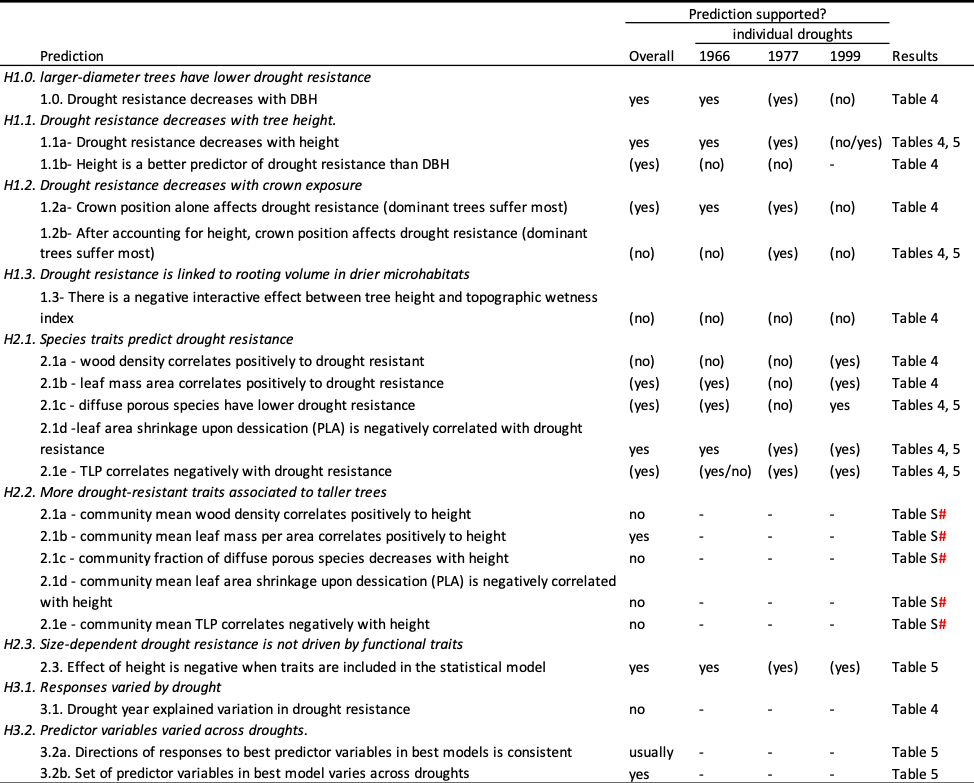
\includegraphics[width=5.20833in]{tables_figures/Table1.png}

We count predictions as fully supported (or rejected) when the direction
of response matches (or contradicts) the prediction. H2.3-H3.2 are based
on if models containing species traits in H2.1 had dAIC\textgreater{}=2
relative to the appropriate null model or to any alternative
multivariate model within 2 dAIC. Parentheses indicate that predictions
were partially supported (or rejected). In other words, parentheses
indicate when the direction of response matched (or contradicted) the
prediction in some but not all models with dAIC\textless{}2 relative to
the appropriate null model. With categorical variables such as crown
position, a ``(yes)'' notation describes when the trend matched the
prediction, but it wasn't significant A ``(yes/no) or (''no/yes``)''
indicates tendencies in opposite directions in univariate tests versus
the best full models, respectively. ``(yes)

\subsubsection{Materials and Methods}\label{materials-and-methods}

\emph{Study site} Research was conducted at the 25.6 ha ForestGEO
(Global Earth Observatory) study plot at the Smithsonian Conservation
Biology Institute (SCBI) in Virginia, USA (38°53'36.6``N, 78°
08'43.4''W) \citep{andersonteixeira_ctfs-forestgeo:_2015}. SCBI is
located in the central Appalachian Mountains at the northern edge of
Shenandoah National Park. Elevations range from 273-338m above sea level
\citep{gonzalezakre_patterns_2016} with a topographic relief of 65m
\citep{bourg_initial_2013}. Dominant species include \emph{Liriodendron
tulipifera}, oaks (\emph{Quercus} spp.), and hickories (\emph{Carya}
spp.).

\emph{Data collection and preparation} The SCBI ForestGEO plot was
censused in 2008, 2013, and 2018 following standard ForestGEO protocols,
whereby all free-standing woody stems \textgreater{}= 1cm diameter at
breast height (DBH) were mapped, tagged, measured at DBH, and identified
to species \citep{condit_tropical_1998}. From this census data, we used
measurements of DBH from 2008 to calculate historical DBH (described
below), along with tree location in the plot to determine the
topographic wetness index. Furthermore, we used data for all stems
\textgreater{}= 10cm to analyze functional trait composition relative to
tree height. \emph{I added the last sentence-- not sure if you've
described that below yet. I don't think you need to note here which data
we use, so long as that's described in the portions where you describe
the analysis.}

We analyzed tree-ring data from the twelve species contributing most to
woody aboveground net primary productivity (ANPP), which together
comprised 97\% of study plot ANPP between 2008 and 2013
\citep{helcoski_growing_2019}. Cores were obtained in 2010-2011 or
2016-2017 from a breast height of 1.3m using a 5mm increment borer. In
2010-2011, cores were collected from randomly selected live trees of
species with at least 30 individuals of DBH \textgreater{}= 10cm
\citep{bourg_initial_2013}. In 2016-2017, cores were collected from all
trees found dead in the annual mortality census
\citep{gonzalezakre_patterns_2016}. Cores were sanded, measured, and
cross-dated using standard procedures, as detailed in
\citep{helcoski_growing_2019}. The resulting chronologies have been
published in association with \citet{helcoski_growing_2019}: (ITRDB;
GitHub/Zenodo). \emph{is this a database? Yes. Ryan submitted the data
but I don't think its posted yet. We should also cite GitHub/Zenodo
here. I'll come back to that. }

Height measurements (n=\# trees) were taken by several researchers
between 2012 to 2019, and are archived in a public
\href{https://github.com/SCBI-ForestGEO/SCBI-ForestGEO-Data/tree/master/tree_dimensions/tree_heights}{GitHub
repository}. Measurement methods included manual
\citep[NEON]{stovall_assessing_2018}, digital rangefinders
\citep{andersonteixeira_size-related_2015}, and automatic LiDAR
\citep{stovall_terrestrial_2018}. Rangefinders either used the tangent
method (Impulse 200LR, TruPulse 360R) or the sine method (Nikon
ForestryPro) for calculating heights. The associated errors for using
either method were acknowledged \citep{larjavaara_measuring_2013}.
Species-specific height allometries were developed (Table S\# -
\textbf{ADD THIS TABLE TO SI}). For species that didn't have enough
height measurements, heights were calculated from equations derived from
all species in the study.

For each tree, we combined tree-ring records and allometric equations of
height and bark thickness to retroactively calculate DBH and estimate
height for the years 1950-2009. Prior DBH was estimated using the
following equation, using 2008 as the earliest year for having reliable
DBH measurements:

\[ diamYEAR = dbh2008 - 2*(bark.depth2008) - 2*\Sigma(ring.widthYEAR:ring.width2008) + 2*(bark.depthYEAR) \]

Here, \emph{ring.width} was measured from cores. Bark thickness was
estimated from species-specific allometries based on the bark thickness
data of \citep{andersonteixeira_size-related_2015}. Specifically, we
used linear regression equations on log-transformed data to relate bark
thickness to DBH (Table S\#- \textbf{create table to give these
equations in SI}) and then used these to estimate bark thickness based
on DBH.

Crown positions were recorded in the field during the growing season of
2018 following the crown position protocol from
\citep{jennings_assessing_1999}, whereby positions were ranked as
dominant, codominant, intermediate, or suppressed. As there was no way
to retroactively estimate crown position, we assumed that 2018 crown
position was reflective of each tree's position over the past 60 years.
While some trees undoubtedly changed position, an analysis of crown
position relative to height (Fig. XX) and height change since
\emph{1959} indicated that change was likely slow. {[}\textbf{work on
this-- provide details?}{]}

Topographic wetness index (TWI) was calculated using the
\citep{R-dynatopmodel} package in R.

\begin{figure}[htbp]
\centering
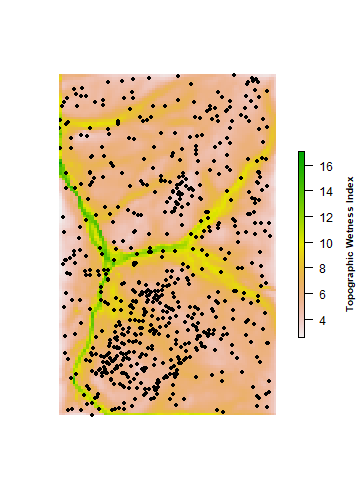
\includegraphics[width=5.20833in]{tables_figures/Figure3.png}
\caption{Location of cored trees}
\end{figure}

Hydraulic traits were collected from SCBI and are summarized in Table 1.
In August 2018, we collected leaf samples from three individuals of each
species \ldots{} (\textbf{Nobby's description of methods for the
following (see word document}) 1. PLA 2. LMA 4. Wood density 5. TLP

\textbf{Table 2. Species analyzed here, listed in descending order of
ANPP\_stem. n cores and DBH range represented, and species traits}
{[}*This replaces/combines the two remaining tables in this section.
Suggested columns, with those to include only if they fit in
parentheses: species, (stems \textgreater{}=10 cm per ha in plot),
(ANPP\_stem), n cores, DBH range of cores, (n cores in each crown
position) species means for each trait{]}

\begin{verbatim}
## Warning: package 'kableExtra' was built under R version 3.4.4
\end{verbatim}

\textbackslash{}begin\{table\}{[}!h{]}

\textbackslash{}caption\{\label{tab:Table2}Overview of analyzed species,
detailing DBH mean and range of cored trees, the number of cores
represented by each crown position of each species, and mean hydraulic
trait measurements. Units of measurements are in mm (DBH), \% (PLA),
g/m2 (LMA), MPa (TLP), and g/cm3 (WD).\} \centering

\begin{tabular}{lrrlrrrr}
\toprule
sp & mean\_DBH & range\_DBH & RP & PLA & LMA & TLP & WD\\
\midrule
caco & 271.87 & 508.0 & ring & 17.22 & 45.86 & -2.13 & 0.83\\
cagl & 313.89 & 887.0 & ring & 21.09 & 42.76 & -2.13 & 0.62\\
caovl & 352.87 & 511.0 & ring & 14.80 & 47.60 & -2.48 & 0.96\\
cato & 209.74 & 201.1 & ring & 16.56 & 45.36 & -2.20 & 0.83\\
fagr & 235.11 & 960.0 & diffuse & 9.45 & 30.68 & -2.57 & 0.62\\
\addlinespace
fram & 353.63 & 883.3 & ring & 13.06 & 43.28 & -2.10 & 0.56\\
juni & 481.42 & 628.0 & semi-ring & 24.64 & 72.13 & -2.76 & 1.09\\
litu & 368.54 & 904.0 & diffuse & 19.56 & 46.92 & -1.92 & 0.40\\
qual & 471.51 & 677.0 & ring & 8.52 & 75.80 & -2.58 & 0.61\\
qupr & 422.48 & 767.0 & ring & 11.75 & 71.77 & -2.36 & 0.61\\
\addlinespace
quru & 548.79 & 1369.3 & ring & 11.01 & 71.13 & -2.64 & 0.62\\
quve & 541.38 & 981.8 & ring & 13.42 & 48.69 & -2.39 & 0.65\\
\bottomrule
\end{tabular}

\textbackslash{}end\{table\}

\emph{Climate and drought years} {[}\textbf{add description of climate
data used in Fig. 1, NEON vertical profiles}{]}

To accurately understand climate sensitivity, this study used a specific
definition of drought, which is not a common practice
\citep{slette_how_2019}. We used the pointRes package \citep{R-pointRes}
in R (version 3.5.3) to determine drought periods based on trees'
drought resistance, which is defined by \citep{lloret_components_2011}
as the ratio between the performance during and before the disturbance.
Candidate drought years were defined if \textgreater{}50\% of the cored
trees experienced \textless{}30\% growth in a year compared to the
previous 5 years. These were then cross-validated with the regional
Palmer Drought Severity Index (PDSI) values for each year, which yielded
a set of three periods that were consistently shown as drought:
1964-1966, 1977, and 1999.

\subsubsection{Results}\label{results}

Results outline

Descriptions of Droughts

\begin{itemize}
\tightlist
\item
  physical characteristics of drought: duration, min PDSI (and when
  occurred), see slette et al 2019 to see how they suggest reporting
  each one
\item
  sum nb.series for each scenario, mult by perc.neg (pointers df),
  define thresholds (e.g.~75\% of all trees experienced the growth
  reduction of 40\% or more)
\item
  make table for this
\item
  citing table 3 (the coefficient for individual year) - maybe mention
  how 77 and 99 have neg coefficients, indicating potential height
  effect: as time goes on, trees are more affected by drought anyways
  because they grow taller
\item
  this is followed by Figure 2
\end{itemize}

Hypothesis results - one header for each main question - present results
for each one, walk through via order and logic of Table 1 - no citations
here

Once the data was collected, linear mixed models were run following the
order of the hypotheses as seen in Figure ???
{[}individual\_tested\_traits{]}. Using the \citep{R-pointRes} package,
we set up models with the resistance value as the response variable, and
each prediction's variable as the independent variable. Variables'
importance in predicting drought tolerance was calculated from
mixed-effects models and the lowest AICc
\citep[\citet{R-AICcmodavg}]{R-lme4}.Null models were determined in
order of the predictions. First, we analyzed the combined scenario to
determine if ``year'' was significant. Upon establishing this, we tested
height and DBH as size parameters. Although both were significant,
height was kept due to its larger delta AICc compared with the null
model. We then tested the remaining biophysical and hydraulic traits
individually against a null model containing height and year. This
yielded Figure ??? (cand\_full). All variables with dAICc
\textgreater{}2 were used as candidates for each scenario's best model
(figure ???? (tested\_traits\_best))

\textbf{Describe each individual drought scenario } 1964-1966 1977 1999

\textbf{Figure 1. Time series of peak growing season (May-August)
climate conditions and residual chronologies for each species.} Droughts
analyzed here are indicated by dashed lines, and shading indicates the
pre-drought period used in calculations of the resistance metric. Figure
modified from \citep{helcoski_growing_2019}.

\begin{figure}[htbp]
\centering
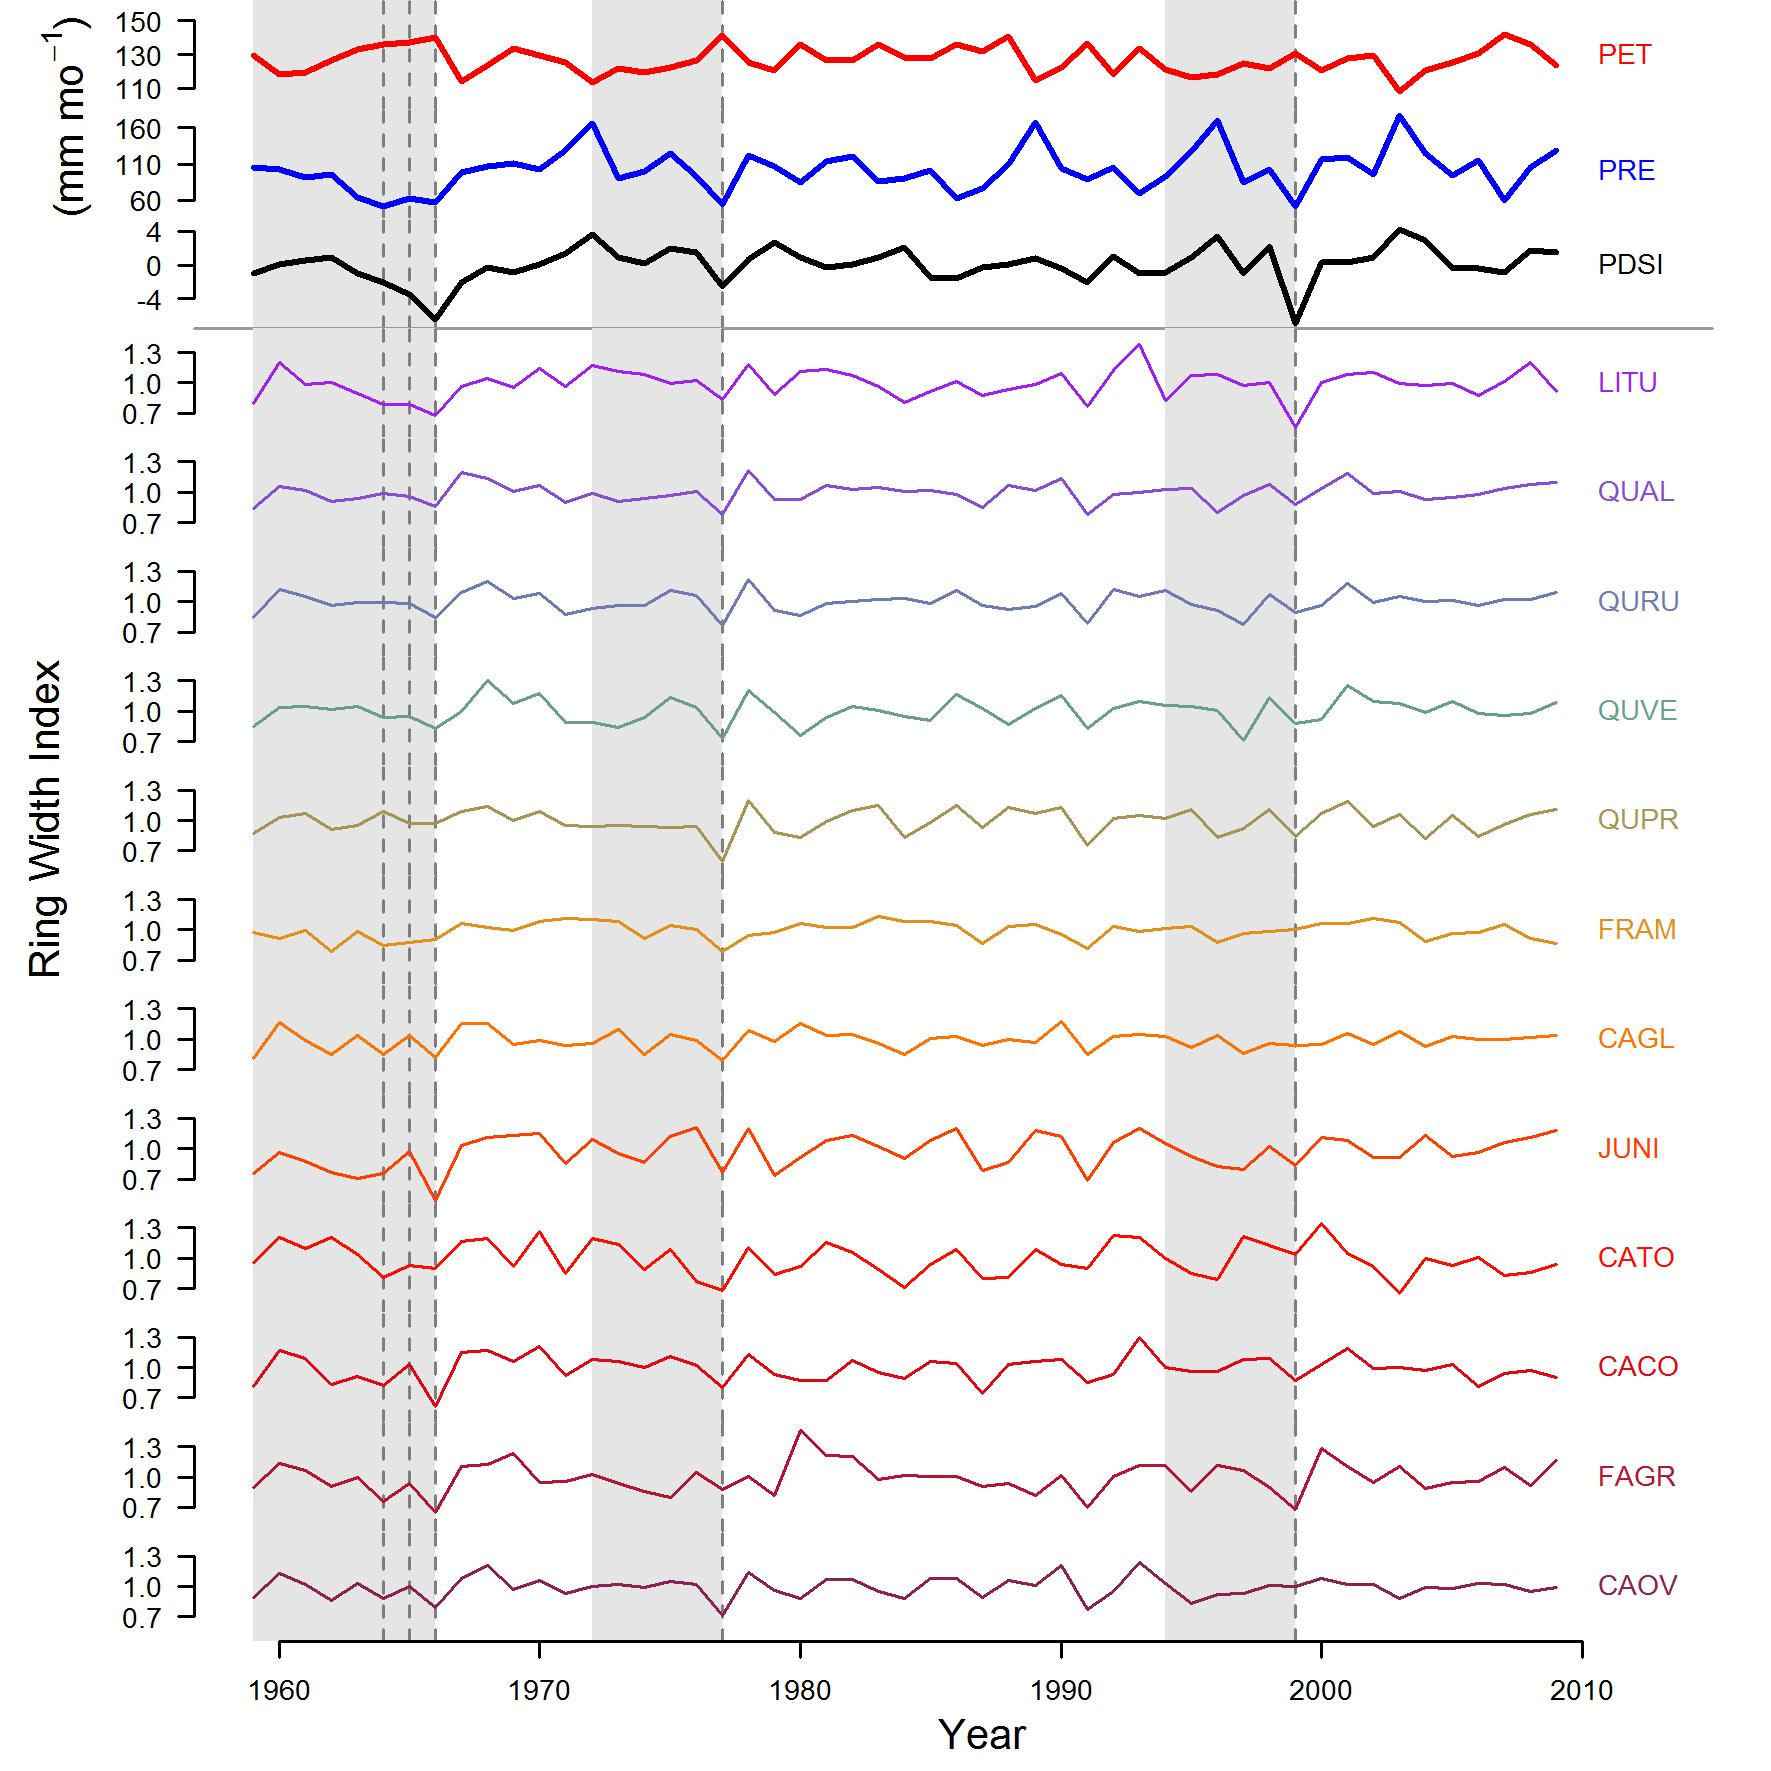
\includegraphics[width=5.20833in]{tables_figures/Figure1.jpg}
\caption{Time series of combined tree cores by species}
\end{figure}

\textbf{Results for first main question: what drives the observed
tendency for large trees to suffer more during drought?} H1.0, H1.1,
H1.2, H1.3 DBH, height, crown position, and TWI

\begin{figure}[htbp]
\centering
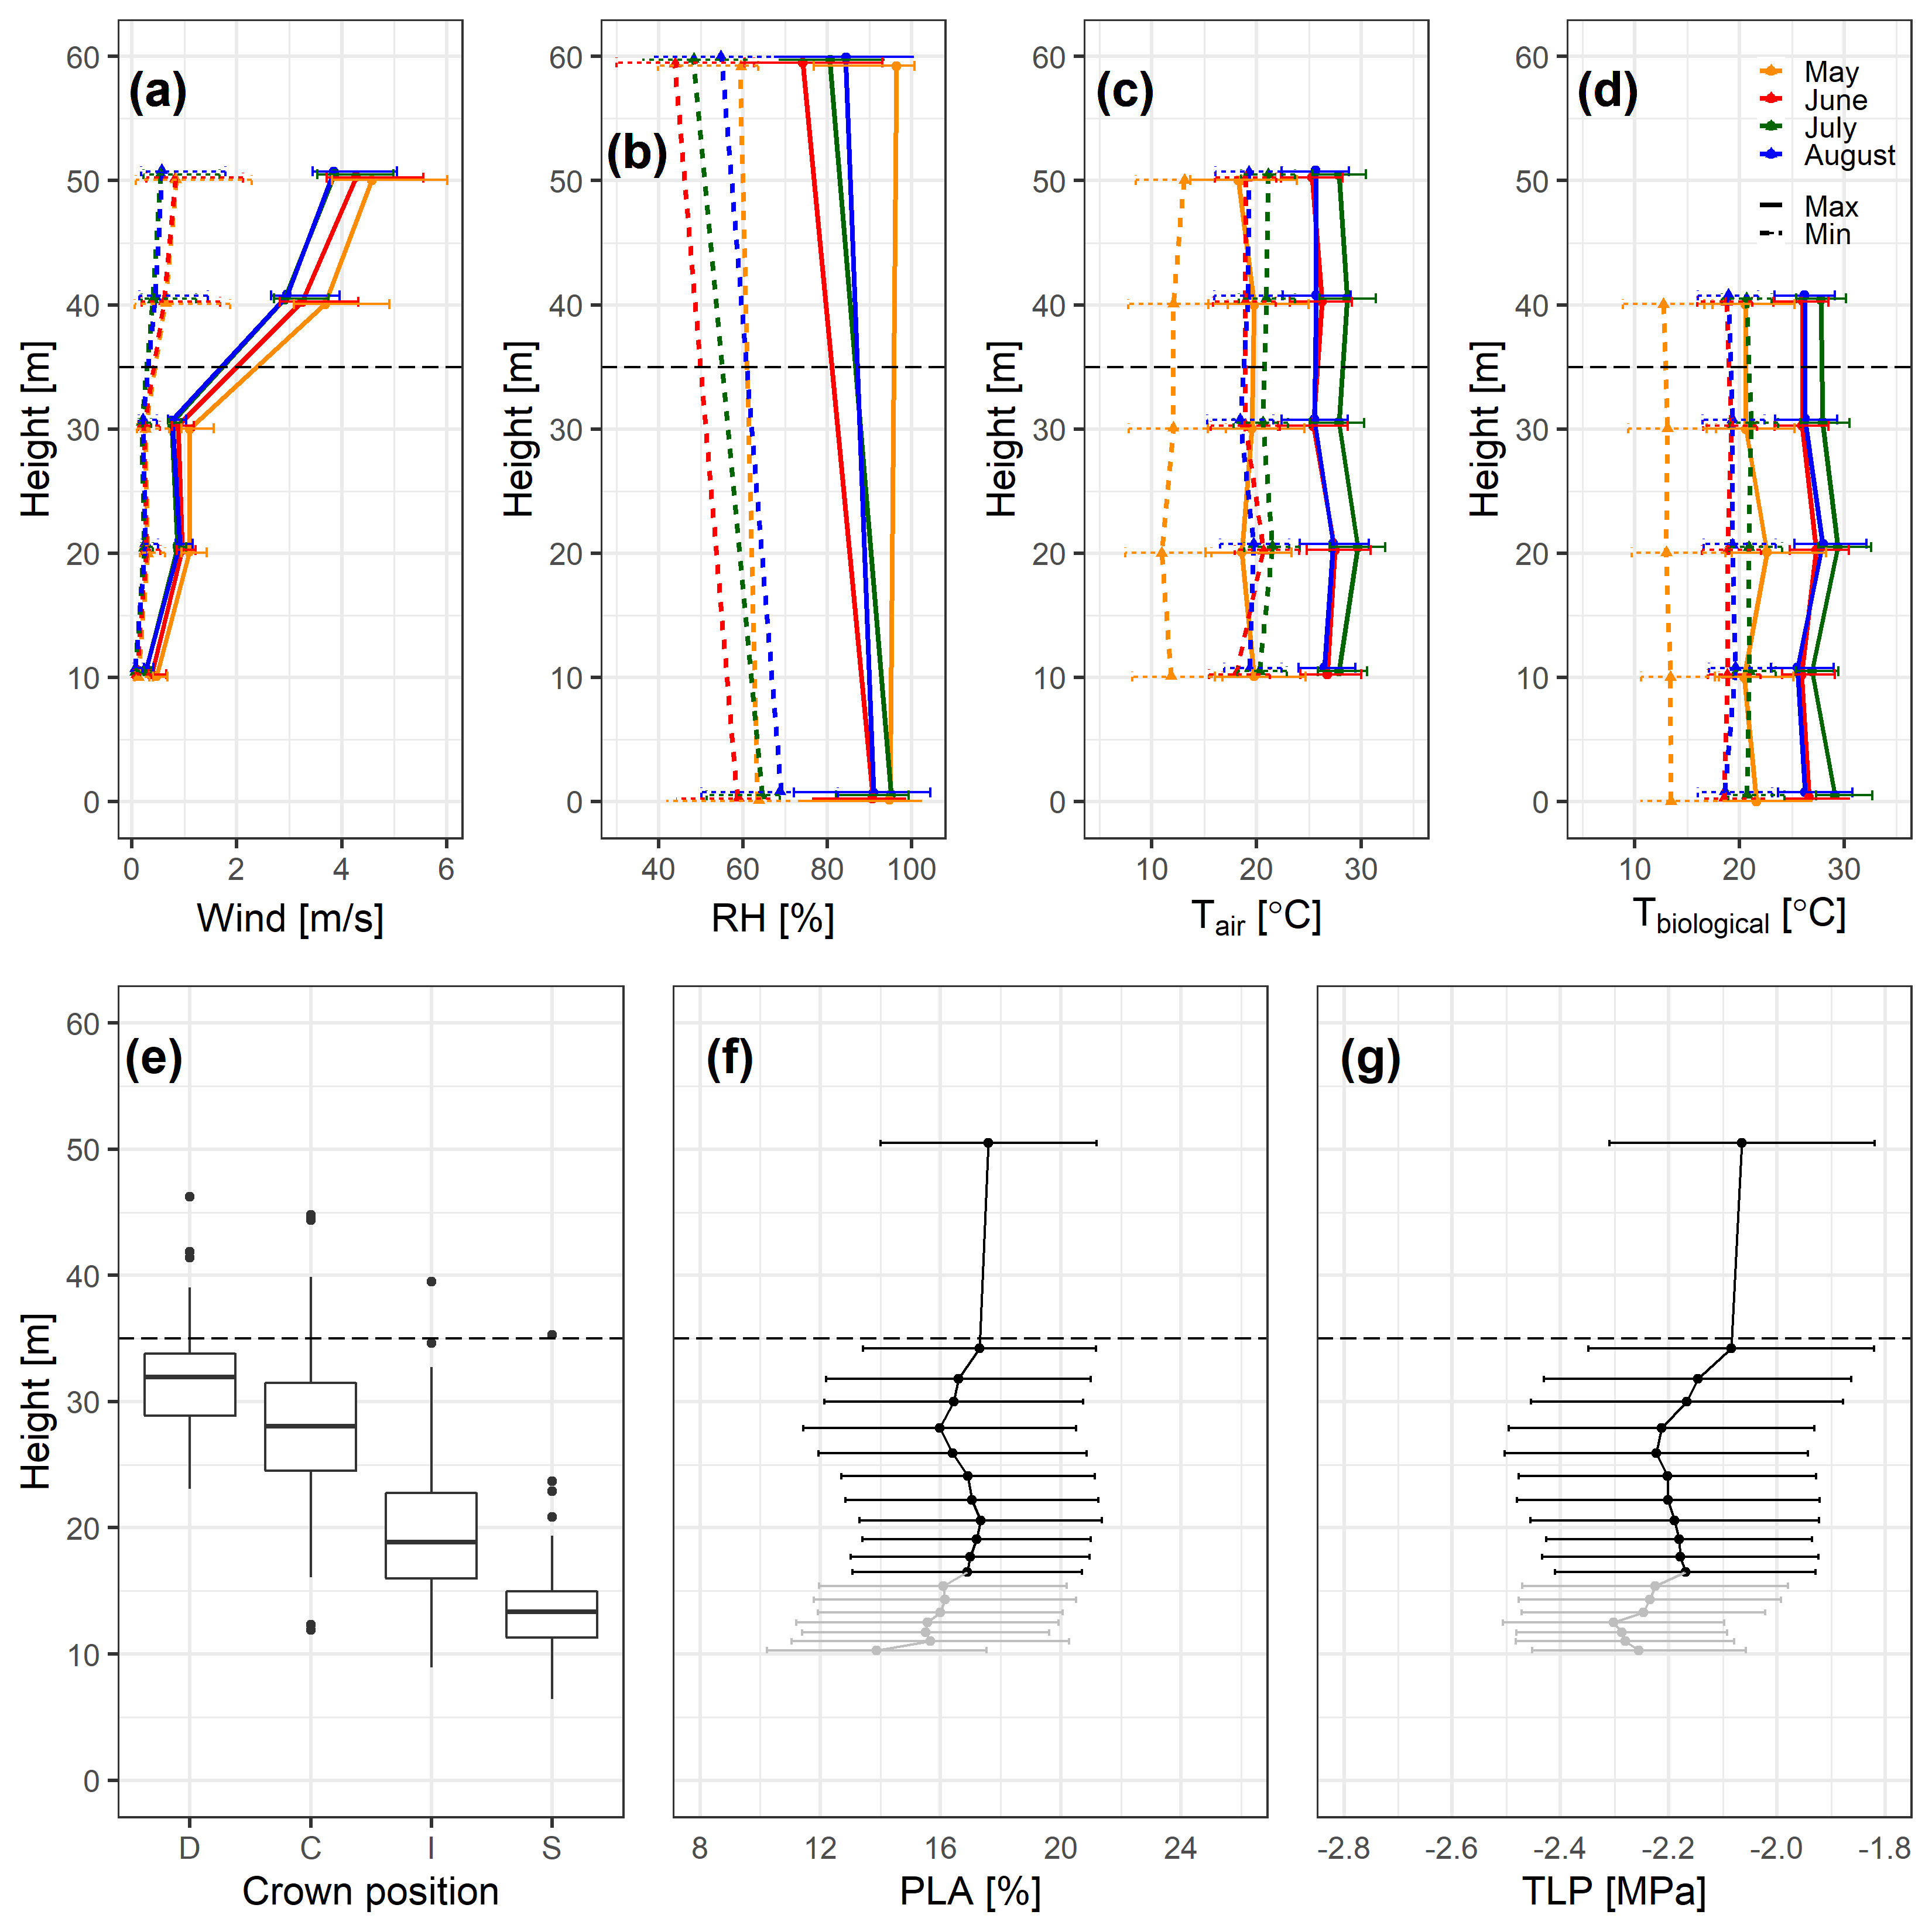
\includegraphics[width=5.20833in]{tables_figures/Figure2.png}
\caption{Height profile graphs}
\end{figure}

\textbf{Results for second main question: how do species' traits - alone
and in interaction with tree size - influence drought response? } H2.1,
H2.2, H2.3 Hydraulic traits alone, traits with height

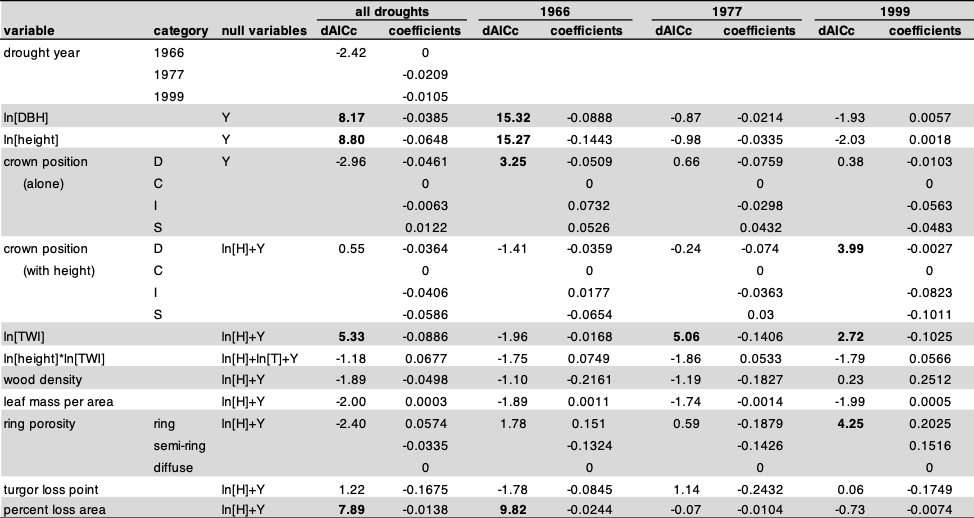
\includegraphics{tables_figures/Table4.png} \#this is
tested\_traits\_all

\textbf{Results for third main question: are responses similar or
variable across individual drought years?} H3.1 and H3.2 Combining
biophysical with hydraulic traits, which come out as candidates for best
model?

\subsubsection{Discussion}\label{discussion}

Discussion outline

\begin{itemize}
\tightlist
\item
  first paragraph is summary of main findings, not re-presenting the
  results
\item
  ``we supported this hypothesis, but not this one'' (following same
  order as Table 1 still)
\item
  direction of responses seems to be relatively consistent but the
  individual responses vary
\item
  tie things in (see here
\item
  main thing is that we're now better understanding what confers
  vulnerability or resilience on trees during drought - how forests
  respond to future droughts/climate change
\item
  ``we filled the gap'' = 1-2 sentences
\item
  limitations at our site:
\item
  aren't able to analyze historical forest community, nor trees that
  were killed by these droughts {[}aka we don't have data for
  individuals that were most severely affected{]} (though we found that
  there's little variation in climate sensitivity for trees that were
  cored dead vs cored alive).
\item
  p50/p80
\item
  We used crown position despite its uncertainty. However, height and
  crown position change relatively slowly so it shouldn't be that far
  off.
\item
  We did not use crowding index because it has much more uncertainty
\item
  limitations for extrapolating other sites:
\item
  forests are different from place to place, but we've seen how in
  forests around the world, forests tend to suffer more. We've
  identified some facets for why this happens. (cite other studies)
\item
  has been observed elsewhere that individuals in more moist habitats
  are more susceptible to drought (cite other studies)
\item
  the species may be different from other sites but the hydraulic traits
  are general across species;
\item
  next paragraph saying that our study advances understanding of
  droughts, e.g.~bennett et al 2015 doesn't go into mechanisms but we do
\item
  and we show that height is more important than exposure, but doesn't
  eliminate the effect of it
\item
  further contribution is we show that two leaf hydraulic traits -
  relatively easy to measure - are good predictors of drought response,
  can be helpful for scaling up (e.g.~from our site to eastern deciduous
  biome)
\item
  biophysical mechanisms are things that should be seen as universal but
  relative importance of each can vary within each drought
\item
  first study to show how these traits affect woody growth response to
  drought \textbf{confirmed by Lawren}
\item
  science is better now. by advancing our understanding of the
  mechanisms for individual-level responses to drought, this opens door
  for better predictions (elaborate from above). ``This is absolutely
  critical to predicting forest responses to future droughts, which
  we're likely to see more of in the future as a result to climate
  change. Forecasting forest responses to these droughts is a huge and
  important challenge'', science is better.
\end{itemize}

\emph{1. paragraph summarizing main results--\textgreater{} primary
conclusions} When including only biophysical traits, trees' resistance
value (on a per-species basis) is explained best by crown position and
height, with codominant trees being the most resistant to drought. This
follows on work done by \citep{bennett_larger_2015} {[}and others?{]}
which show that larger trees suffer more during drought, and confirms
that this susceptibility can be seen in tree ring analyses. Adding in
crown position with the leaf hydraulic traits yields a slightly worse
predictive model for drought tolerance, with height remaining as the
only significant biophysical variable.

We partially supported the hypothesis that crown exposure makes trees
more vulnerable to drought. Co-dominant trees had the highest drought
resistance. Dominant trees had lower resistance, likely because they are
the most exposed. Other studies have found clear evidence of greater
drought sensitivity in trees with exposed crowns (e.g.,
\citep{suarez_factors_2004}; \citep{scharnweber_confessions_2019}). At
the same time, intermediate and suppressed trees had even lower
resistance. This indicates that other mechanisms such as competition or
rooting depth were important. (Also note that our study design was not
ideal for testing the role of canopy position. Current canopy position
is a conservative separator of canopy position: trees may currently be
in more dominant positions than they were at the time, but backwards
movement is unlikely. This would bias against finding a signficant
effect for H1.2. Height may be a more reliable predictor of past canopy
position than is current canopy position, and explains a portion of
variation in canopy position.)

Proximity to stream--either vertical (elev) or horizontal (distance)--
did not increase drought resistance; rather, it tended to decrease
resistance (H1.3a). This may be because individuals growing further from
water are acclimatized to drier conditions. However, the increase in
drought resistance with distance from stream was less for small than
large trees (H1.3b), indicating a potential importance of root
depth/volume in conferring drought resistance.

\textbf{misc content to integrate} From \citep{kannenberg_linking_2019},
species with diffuse porous wood anatomy (\emph{Liriodendron}) are more
sensitive to drought, whereas ring-porous are not as affected because
they more easily rebuild structures for hydraulic conductivity. This
paper mentions it would be good to have this data with respect to latent
affects from drought. \#\#\# Acknowledgements

words

\subsubsection{Author Contribution}\label{author-contribution}

words

\subsubsection{Supplementary
Information}\label{supplementary-information}

\begin{table}[!h]

\caption{\label{tab:Table S1}Species-specific height regression equations}
\centering
\begin{tabular}{llr}
\toprule
Species & Equations & r.2\\
\midrule
Carya cordiformis & 0.348+0.808*x & 0.879\\
Carya glabra & 0.681+0.704*x & 0.855\\
Carya ovalis & 0.621+0.722*x & 0.916\\
Carya tomentosa & 0.776+0.701*x & 0.894\\
Fagus grandifolia & 0.708+0.662*x & 0.857\\
\addlinespace
Liriodendron tulipifera & 1.32+0.524*x & 0.761\\
Quercus alba & 1.14+0.548*x & 0.647\\
Quercus prinus & 0.44+0.751*x & 0.869\\
Quercus rubra & 1.17+0.533*x & 0.773\\
all & 0.879+0.634*x & 0.857\\
\bottomrule
\end{tabular}
\end{table}

\emph{p50 and p80} We decided to include values of P50 and P80 in the
leaf traits model, defined by \citep{anderegg_meta-analysis_2016} as the
water potentials at which a species loses 50\% and 88\% {[}80\% by
proxy{]}, respectively, of hydraulic conductivity. Values were
calculated by (\textbf{insert new methods here??}), and were only
available for six species (\emph{C. glabra}, \emph{L. tulipifera},
\emph{Q. alba}, \emph{Q. prinus}, \emph{Q. rubra}, and \emph{Q.
velutina}). Because of this, the model runs were considered to be
incomplete due to the exclusion of the other 8 species. Results revealed
neither p50 nor p80 to be significant, thus for the full analysis we
decided to drop the two traits in order to include all species in the
full analysis.

\begin{table}[!h]

\caption{\label{tab:Table S2}Candidate variables for best model}
\centering
\begin{tabular}{rlll}
\toprule
prediction & variable & variable\_description & top\_model\\
\midrule
1.2 & position\_all & crown.position w/height & 1999\\
2.2 & height.ln.m & ln[height] & all\\
2.2 & height.ln.m & ln[height] & 1966\\
2.3 & position\_all & crown.position alone & 1966\\
2.4 & TWI.ln & ln[topographic.wetness.index] & all\\
\addlinespace
2.4 & TWI.ln & ln[topographic.wetness.index] & 1977\\
2.4 & TWI.ln & ln[topographic.wetness.index] & 1999\\
3.1 & year & drought.year & all\\
3.1 & rp & ring.porosity & 1999\\
3.2 & PLA\_dry\_percent & percent.loss.area & all\\
\addlinespace
3.2 & PLA\_dry\_percent & percent.loss.area & 1966\\
3.4 & mean\_TLP\_Mpa & mean.turgor.loss.point & all\\
\bottomrule
\end{tabular}
\end{table}

\begin{figure}[ht]
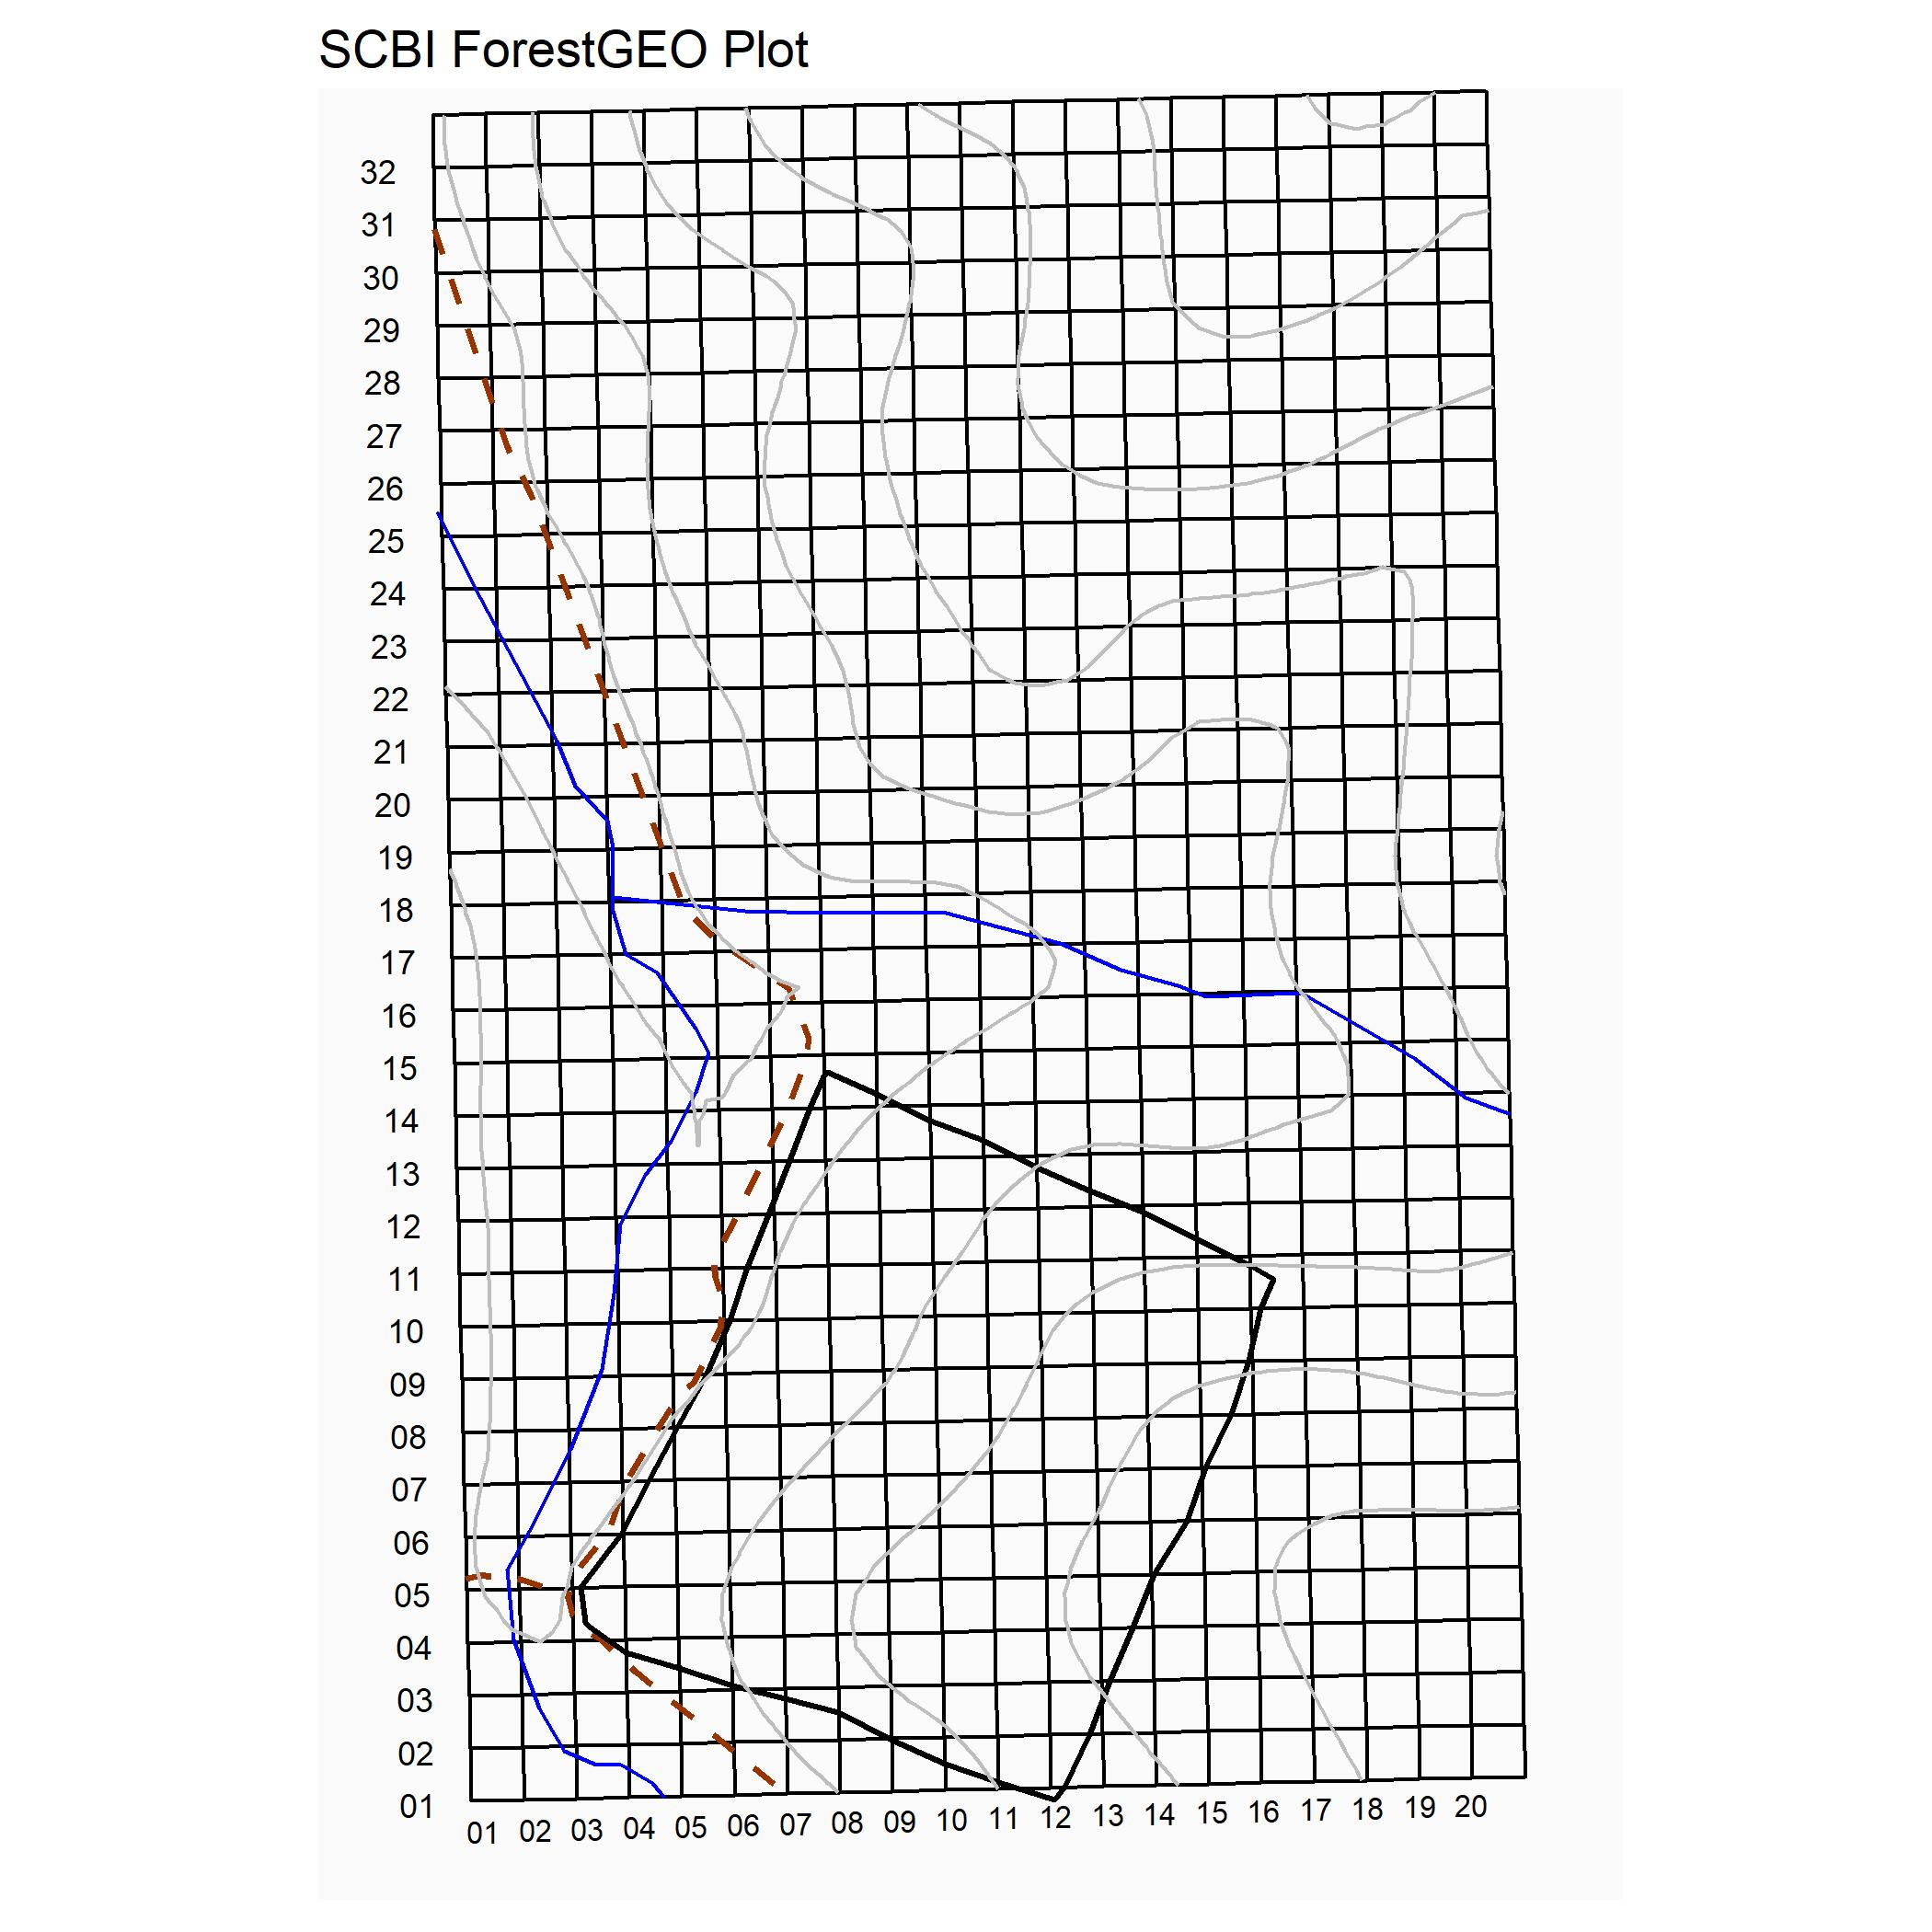
\includegraphics[width=1\linewidth]{tables_figures/ForestGEO_plot} \caption{Map of ForestGEO plot}\label{fig:Plot}
\end{figure}

\emph{how do we want to present Table S3? Would it be better as an image
of an excel file, since it's so large? Did we want to keep all
coefficients here?}

\begin{table}[!h]

\caption{\label{tab:Table S3}Top model variations for each drought scenario, with dAICc values <= 2}
\centering
\begin{tabular}{lrll}
\toprule
Modnames & Delta\_AICc & scenario & coef\\
\midrule
resist.value \textasciitilde{} position\_all+height.ln.m+TWI.ln+year+PLA\_dry\_percent+mean\_TLP\_Mpa+(1|sp/tree) & 0.00 & trees\_all\_sub & (Intercept) (1.101), position\_alldominant (-0.044), position\_allintermediate (-0.039), position\_allsuppressed (-0.049), height.ln.m (-0.092), TWI.ln (-0.058), year1977 (-0.088), year1999 (-0.073), PLA\_dry\_percent (-0.008), mean\_TLP\_Mpa (-0.148)\\
resist.value \textasciitilde{} height.ln.m+TWI.ln+year+PLA\_dry\_percent+mean\_TLP\_Mpa+(1|sp/tree) & 0.84 & trees\_all\_sub & (Intercept) (0.953), height.ln.m (-0.06), TWI.ln (-0.065), year1977 (-0.089), year1999 (-0.076), PLA\_dry\_percent (-0.008), mean\_TLP\_Mpa (-0.164)\\
resist.value \textasciitilde{} position\_all+height.ln.m+year+PLA\_dry\_percent+mean\_TLP\_Mpa+(1|sp/tree) & 1.57 & trees\_all\_sub & (Intercept) (1.021), position\_alldominant (-0.046), position\_allintermediate (-0.042), position\_allsuppressed (-0.053), height.ln.m (-0.097), year1977 (-0.088), year1999 (-0.073), PLA\_dry\_percent (-0.009), mean\_TLP\_Mpa (-0.146)\\
resist.value \textasciitilde{} height.ln.m+rp+PLA\_dry\_percent+(1|sp) & 0.00 & x1966 & (Intercept) (1.576), height.ln.m (-0.145), rpring (0.091), rpsemi-ring (0.232), PLA\_dry\_percent (-0.021)\\
resist.value \textasciitilde{} height.ln.m+TWI.ln+rp+PLA\_dry\_percent+(1|sp) & 1.37 & x1966 & (Intercept) (1.505), height.ln.m (-0.146), TWI.ln (0.043), rpring (0.092), rpsemi-ring (0.227), PLA\_dry\_percent (-0.021)\\
\addlinespace
resist.value \textasciitilde{} height.ln.m+PLA\_dry\_percent+mean\_TLP\_Mpa+(1|sp) & 1.39 & x1966 & (Intercept) (1.177), height.ln.m (-0.135), PLA\_dry\_percent (-0.014), mean\_TLP\_Mpa (-0.148)\\
resist.value \textasciitilde{} TWI.ln+rp+mean\_TLP\_Mpa+(1|sp) & 0.00 & x1977 & (Intercept) (0.386), TWI.ln (-0.136), rpring (-0.233), rpsemi-ring (-0.328), mean\_TLP\_Mpa (-0.37)\\
resist.value \textasciitilde{} position\_all+TWI.ln+rp+mean\_TLP\_Mpa+(1|sp) & 0.28 & x1977 & (Intercept) (0.341), position\_alldominant (-0.079), position\_allintermediate (-0.025), position\_allsuppressed (0.039), TWI.ln (-0.128), rpring (-0.23), rpsemi-ring (-0.335), mean\_TLP\_Mpa (-0.385)\\
resist.value \textasciitilde{} height.ln.m+TWI.ln+rp+mean\_TLP\_Mpa+(1|sp) & 1.06 & x1977 & (Intercept) (0.469), height.ln.m (-0.032), TWI.ln (-0.133), rpring (-0.223), rpsemi-ring (-0.318), mean\_TLP\_Mpa (-0.368)\\
resist.value \textasciitilde{} position\_all+height.ln.m+TWI.ln+rp+PLA\_dry\_percent+(1|sp) & 0.00 & x1999 & (Intercept) (1.31), position\_alldominant (0.003), position\_allintermediate (-0.077), position\_allsuppressed (-0.1), height.ln.m (-0.09), TWI.ln (-0.083), rpring (0.191), rpsemi-ring (0.224), PLA\_dry\_percent (-0.009)\\
\addlinespace
resist.value \textasciitilde{} position\_all+height.ln.m+TWI.ln+rp+mean\_TLP\_Mpa+(1|sp) & 0.05 & x1999 & (Intercept) (0.855), position\_alldominant (0.001), position\_allintermediate (-0.078), position\_allsuppressed (-0.1), height.ln.m (-0.092), TWI.ln (-0.08), rpring (0.183), rpsemi-ring (0.06), mean\_TLP\_Mpa (-0.146)\\
resist.value \textasciitilde{} position\_all+height.ln.m+TWI.ln+rp+(1|sp) & 0.55 & x1999 & (Intercept) (1.19), position\_alldominant (0.002), position\_allintermediate (-0.08), position\_allsuppressed (-0.104), height.ln.m (-0.09), TWI.ln (-0.085), rpring (0.199), rpsemi-ring (0.134)\\
resist.value \textasciitilde{} position\_all+height.ln.m+rp+mean\_TLP\_Mpa+(1|sp) & 0.94 & x1999 & (Intercept) (0.722), position\_alldominant (-0.002), position\_allintermediate (-0.083), position\_allsuppressed (-0.105), height.ln.m (-0.1), rpring (0.183), rpsemi-ring (0.046), mean\_TLP\_Mpa (-0.154)\\
resist.value \textasciitilde{} TWI.ln+rp+PLA\_dry\_percent+(1|sp) & 1.07 & x1999 & (Intercept) (1.044), TWI.ln (-0.097), rpring (0.187), rpsemi-ring (0.265), PLA\_dry\_percent (-0.01)\\
resist.value \textasciitilde{} position\_all+height.ln.m+rp+PLA\_dry\_percent+(1|sp) & 1.15 & x1999 & (Intercept) (1.191), position\_alldominant (0.001), position\_allintermediate (-0.081), position\_allsuppressed (-0.106), height.ln.m (-0.098), rpring (0.192), rpsemi-ring (0.215), PLA\_dry\_percent (-0.009)\\
\addlinespace
resist.value \textasciitilde{} TWI.ln+rp+mean\_TLP\_Mpa+(1|sp) & 1.41 & x1999 & (Intercept) (0.516), TWI.ln (-0.094), rpring (0.178), rpsemi-ring (0.074), mean\_TLP\_Mpa (-0.166)\\
resist.value \textasciitilde{} position\_all+height.ln.m+TWI.ln+rp+PLA\_dry\_percent+mean\_TLP\_Mpa+(1|sp) & 1.82 & x1999 & (Intercept) (1.084), position\_alldominant (0.002), position\_allintermediate (-0.077), position\_allsuppressed (-0.099), height.ln.m (-0.091), TWI.ln (-0.081), rpring (0.186), rpsemi-ring (0.147), PLA\_dry\_percent (-0.005), mean\_TLP\_Mpa (-0.076)\\
resist.value \textasciitilde{} position\_all+height.ln.m+rp+(1|sp) & 1.88 & x1999 & (Intercept) (1.065), position\_alldominant (-0.001), position\_allintermediate (-0.085), position\_allsuppressed (-0.11), height.ln.m (-0.098), rpring (0.201), rpsemi-ring (0.123)\\
\bottomrule
\end{tabular}
\end{table}

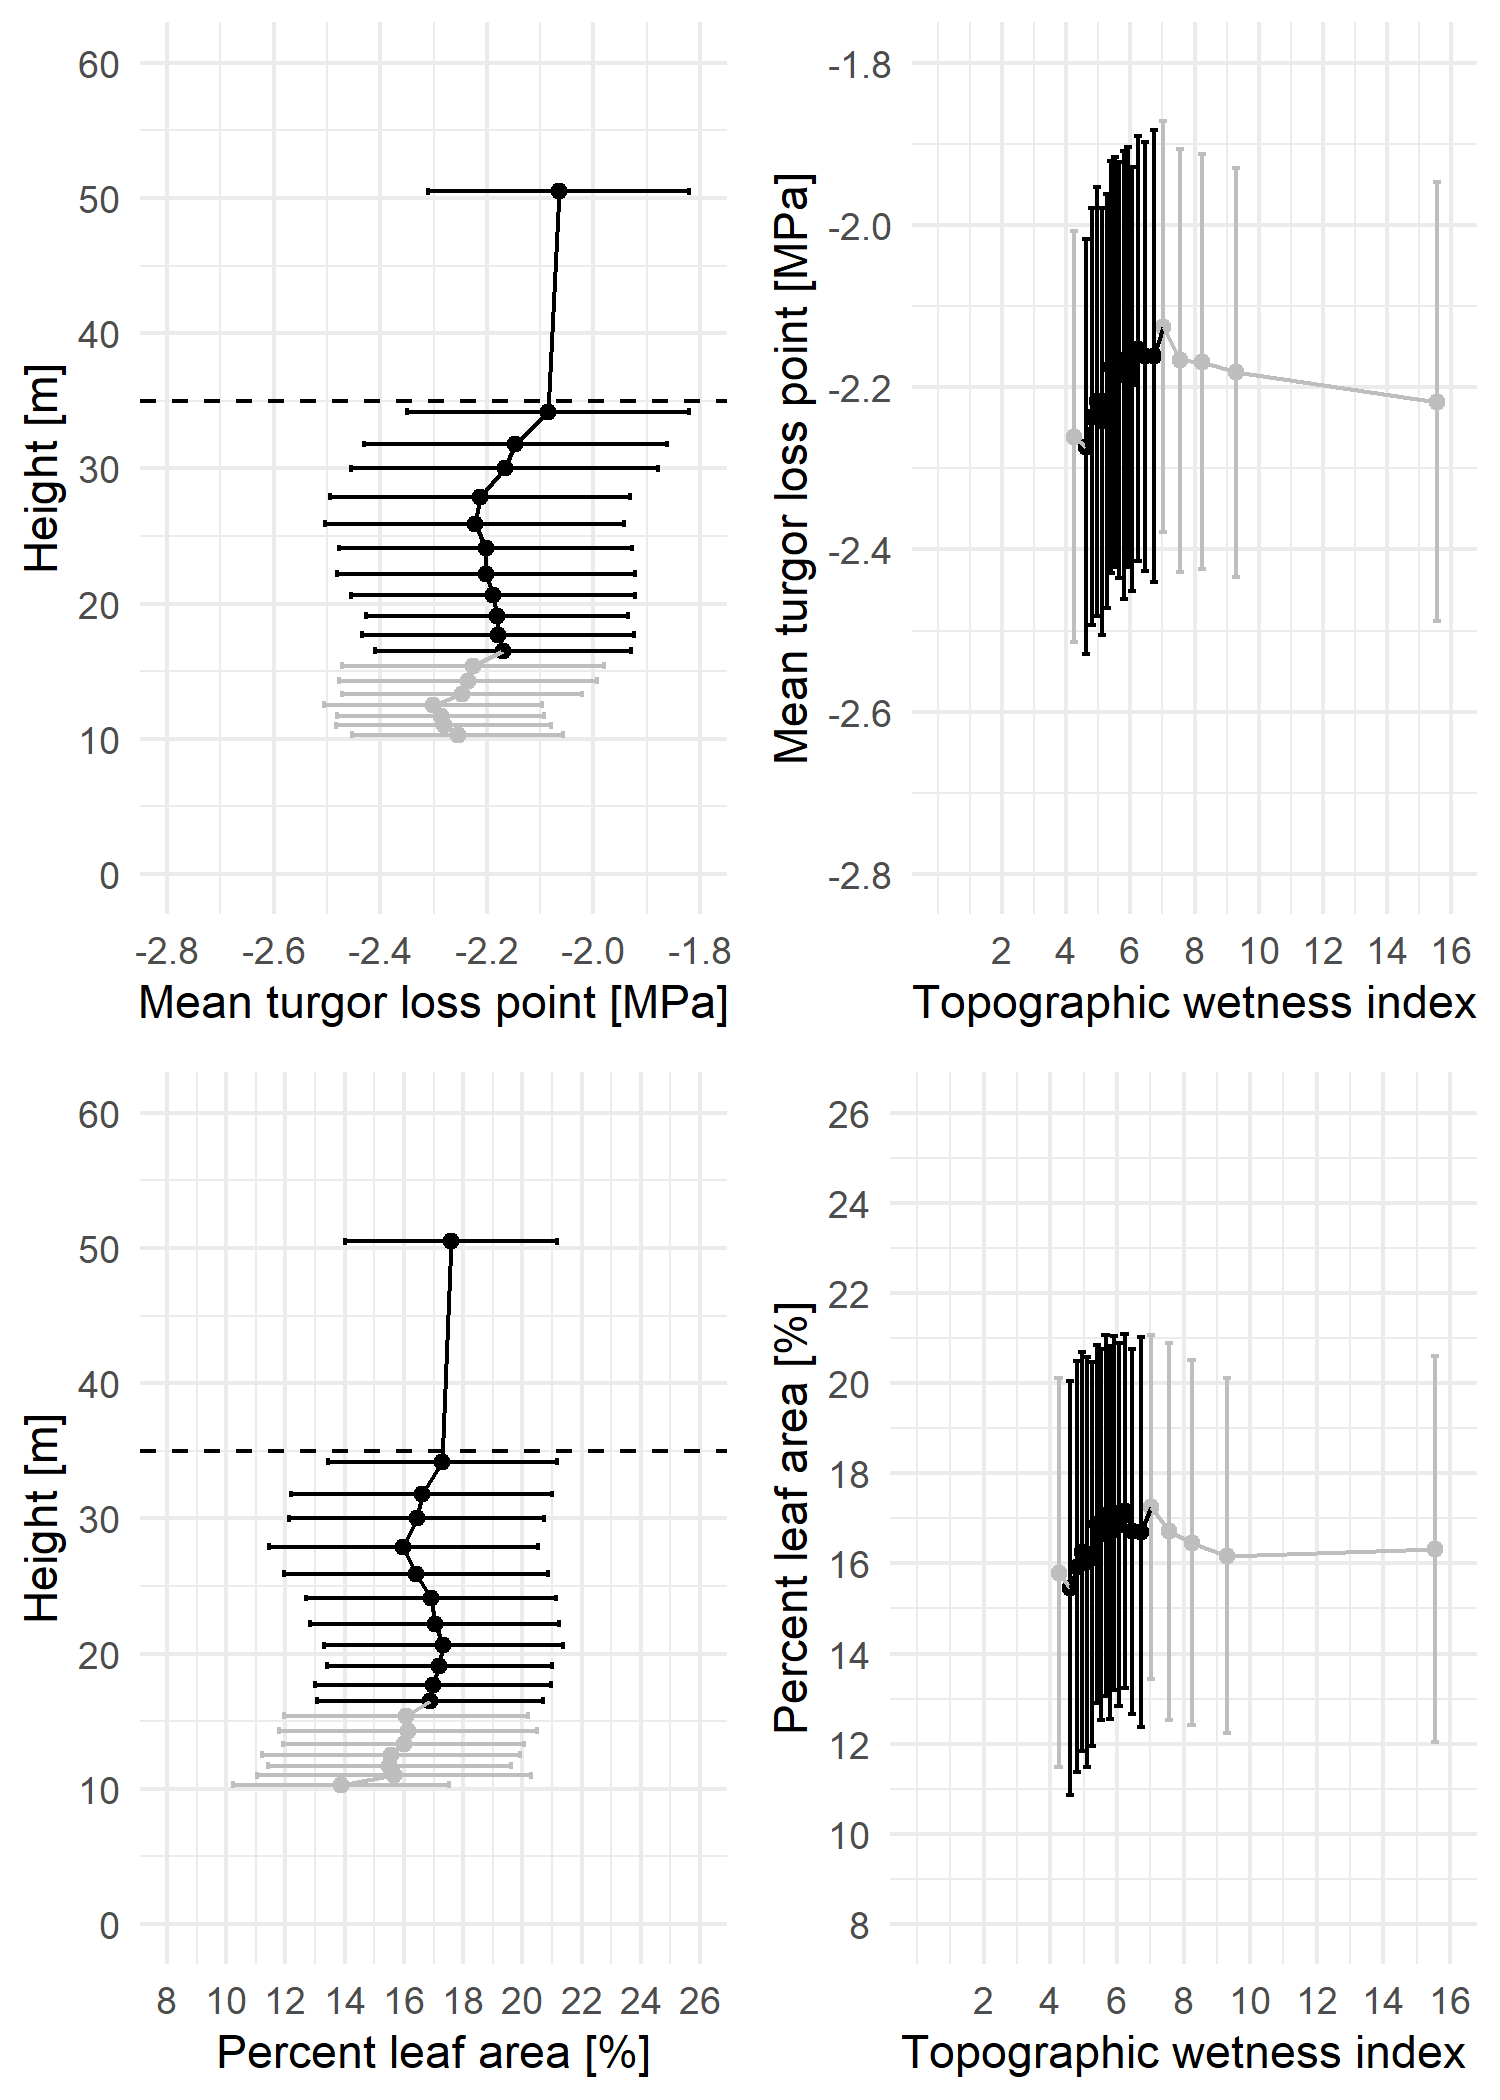
\includegraphics{tables_figures/FigureS1.png} (see Issue \#32)

\bibliography{book.bib,packages.bib}


\end{document}
